\documentclass[]{standalone}
\usepackage{amsmath}
\usepackage{amssymb}
% No page numbers and no paragraph indentation                                  
\pagestyle{empty}                                                               
\setlength{\parindent}{0bp}%
\usepackage{graphicx}
\usepackage{tikz}
\usepackage{xcolor}
\usetikzlibrary{calc,fadings,decorations.pathreplacing,shapes,shapes.multipart,arrows,shapes.misc,intersections,positioning}

\begin{document}

\tikzset{
    partial ellipse/.style args={#1:#2:#3}{
        insert path={+ (#1:#3) arc (#1:#2:#3)}
    }
}

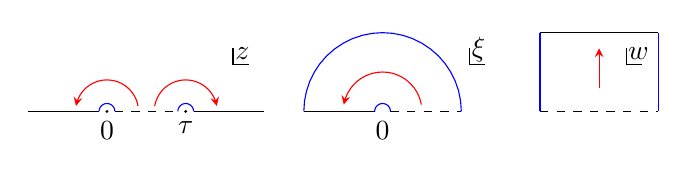
\begin{tikzpicture}[scale = 1]
\draw (0,0) --(0.9,0);
\draw[dashed] (1.1,0)--++(0.8,0);
\draw (2.1,0)--++(.9,0);
\node[below] () at (1,0) {$0$};
\fill (1,0) circle (0.02);
\node[below] () at (2,0) {$\tau$};
\fill (2,0) circle (0.02);
\draw[blue] [domain=0:180] plot ({1+0.1*cos(\x)}, {0.1*sin(\x)});
\draw[blue] [domain=0:180] plot ({2+0.1*cos(\x)}, {0.1*sin(\x)});
\draw[red] [-stealth,domain=10:170] plot ({1+0.4*cos(\x)}, {0.4*sin(\x)});
\draw[red] [-stealth,domain=170:10] plot ({2+0.4*cos(\x)}, {0.4*sin(\x)});
\begin{scope}[shift={(2.6,0.6)}]
\node () at (0.12,0.14) {$z$};
\draw (0,0.2)--(0,0)--(0.2,0);
\end{scope}
\begin{scope}[shift={(3.5,0)}]
\draw (0,0) --(0.9,0);
\draw[dashed] (1.1,0)--++(0.9,0);
\node[below] () at (1,0) {$0$};
\draw[blue] [domain=0:180] plot ({1+0.1*cos(\x)}, {0.1*sin(\x)});
\draw[blue] [domain=0:180] plot ({1+1*cos(\x)}, {1*sin(\x)});
\draw[red] [-stealth,domain=10:170] plot ({1+0.5*cos(\x)}, {0.5*sin(\x)});
\end{scope}
\begin{scope}[shift={(5.6,0.6)}]
\node () at (0.12,0.19) {$\xi$};
\draw (0,0.2)--(0,0)--(0.2,0);
\end{scope}
\begin{scope}[shift={(6.5,0)}]
\draw[dashed] (0,0)--(1.5,0);
\draw[blue] (0,0)--(0,1);
\draw (0,1)--(1.5,1);
\draw[blue] (1.5,1)--(1.5,0);
\draw[-stealth,red] (0.75,0.3)--++(0,0.5);
\end{scope}
\begin{scope}[shift={(7.6,0.6)}]
\node () at (0.15,0.13) {$w$};
\draw (0,0.2)--(0,0)--(0.2,0);
\end{scope}
\end{tikzpicture}


\end{document}